\documentclass{beamer}
\usepackage{pgfpages}
%\setbeameroption{show notes on second screen=left} %enable for notes
\usepackage{graphicx}
\usepackage{xcolor}
\usepackage{listings}
%\usepackage{transparent}
\usepackage{hyperref}
\lstset{language=python,frame=single}
\usepackage{verbatim}
%\usepackage{apacite}
\usepackage[longnamesfirst]{natbib}
\usepackage{subcaption}
\usepackage{amsmath}
\usepackage{relsize}
\usepackage{appendixnumberbeamer}
\usepackage{xparse}
\usepackage{multimedia}
\usepackage{xcolor}
\usepackage[normalem]{ulem}
\usepackage{tikz}
\usetikzlibrary{matrix,backgrounds}
\usetikzlibrary{positioning}
\usetikzlibrary{shapes,arrows}
\usetikzlibrary{positioning}

\tikzset{onslide/.code args={<#1>#2}{%
  \only<#1>{\pgfkeysalso{#2}} 
}}

\tikzstyle{block} = [rectangle, draw, fill=red!20!blue!10, 
    text width=5em, text centered, rounded corners, minimum height=4em]
\tikzstyle{netnode} = [circle, draw, very thick, inner sep=0pt, minimum size=0.5cm] 
\tikzstyle{relunode} = [rectangle, draw, very thick, inner sep=0pt, minimum size=0.5cm] 
    
\tikzstyle{line} = [draw, line width=1.5pt, -latex']

\pgfdeclarelayer{background}
\pgfsetlayers{background,main}

\pgfdeclarelayer{myback}
\pgfsetlayers{myback,background,main}

\usetheme[numbering=fraction]{metropolis}
\newcommand{\semitransp}[2][35]{\color{fg!#1}#2}

\newcommand\blfootnote[1]{%
  \begingroup
  \renewcommand\thefootnote{}\footnote{#1}%
  \addtocounter{footnote}{-1}%
  \endgroup
}
\renewcommand*\footnoterule{}
%%\AtBeginSection[]
%%{
%%  \begin{frame}
%%    \frametitle{Table of Contents}
%%    \tableofcontents[currentsection]
%%  \end{frame}
%%}


\newcommand{\trainerr}{\mathcal{\varepsilon}_\text{train}}
\newcommand{\generr}{\mathcal{\varepsilon}_\text{test}}

\newcommand{\toptn}{{t}^\text{opt}_\text{gradient}}
\newcommand{\eoptn}{\mathcal{\varepsilon}^\text{opt}_\text{gradient}}
\newcommand{\eoptnn}{\mathcal{\varepsilon}^\text{opt}_\text{non-gradient}}

\newcommand{\wa}{{\bf{W}^{21}}}
\newcommand{\wb}{{\bf{W}^{32}}}
\newcommand{\ddt}{\frac{d}{dt}}
\newcommand{\ovn}{\overline{N}}
\newcommand{\rank}{\text{rank}}

\begin{document}

\title{Understanding generalization and transfer in deep linear neural networks}
\author{Andrew Lampinen}
\date{FriSem, 1/18/2019}
\frame{\titlepage}

\begin{frame}{Generalization in deep networks: ``Creativity'' from AlphaGo}
\begin{figure}
\includegraphics[width=0.5\textwidth]{figures/alphago_move_37.png}
\end{figure}
\note{This is a move that nobody has seen before, during the game commentators called it ``probably a mistake,'' but later decided it was ``beautiful.''}
\end{frame}

\begin{frame}{Generalization in humans: Past tense over-regularization}
\begin{figure}
\includegraphics[width=0.8\textwidth]{figures/past_tense.png}
\end{figure}
\note{There are many interesting phenomena like this, but there's a general pattern of learning broad features followed by progressive differentiation of lower level structure.}
\end{frame}

\begin{frame}[standout]
How, why, and when do neural networks (and humans) generalize?
\end{frame}

\begin{frame}{Outline}
\vspace{1em}
\tableofcontents
\end{frame}

\section{The theory}

\subsection{Setup: Deep linear networks}
\begin{frame}{Deep linear networks}
\begin{figure}
\centering
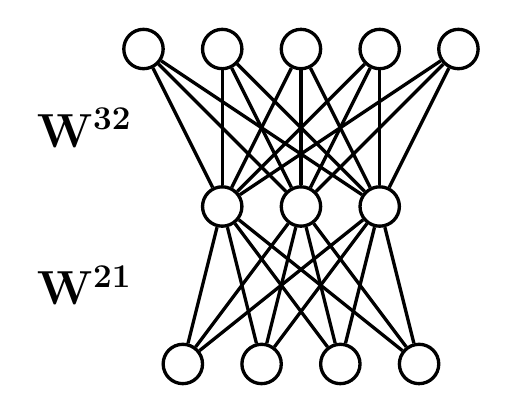
\begin{tikzpicture}[auto]

\node [netnode] at (-1.5,-2) (i1) {};
\node [netnode] at (-0.5,-2) (i2) {};
\node [netnode] at (0.5,-2) (i3) {};
\node [netnode] at (1.5,-2) (i4) {};

\node [netnode] at (-1,0) (h111) {};
\node [netnode] at (0,0) (h112) {};
\node [netnode] at (1,0) (h113) {};

\path [draw, very thick] (i1) to (h111);
\path [draw, very thick] (i1) to (h112);
\path [draw, very thick] (i1) to (h113);
\path [draw, very thick] (i2) to (h111);
\path [draw, very thick] (i2) to (h112);
\path [draw, very thick] (i2) to (h113);
\path [draw, very thick] (i3) to (h111);
\path [draw, very thick] (i3) to (h112);
\path [draw, very thick] (i3) to (h113);
\path [draw, very thick] (i4) to (h111);
\path [draw, very thick] (i4) to (h112);
\path [draw, very thick] (i4) to (h113);

\node [netnode] at (-2,2) (h120) {};
\node [netnode] at (-1,2) (h121) {};
\node [netnode] at (0,2) (h122) {};
\node [netnode] at (1,2) (h123) {};
\node [netnode] at (2,2) (h124) {};

\path [draw, very thick] (h111) to (h120);
\path [draw, very thick] (h111) to (h121);
\path [draw, very thick] (h111) to (h122);
\path [draw, very thick] (h111) to (h123);
\path [draw, very thick] (h111) to (h124);
\path [draw, very thick] (h112) to (h120);
\path [draw, very thick] (h112) to (h121);
\path [draw, very thick] (h112) to (h122);
\path [draw, very thick] (h112) to (h123);
\path [draw, very thick] (h112) to (h124);
\path [draw, very thick] (h113) to (h120);
\path [draw, very thick] (h113) to (h121);
\path [draw, very thick] (h113) to (h122);
\path [draw, very thick] (h113) to (h123);
\path [draw, very thick] (h113) to (h124);


%% annotations

\node at (-2.75, -1) {\LARGE$\wa$};
\node at (-2.75, 1) {\LARGE$\wb$};

\end{tikzpicture}
\end{figure}


\end{frame}

\subsection{Learning dynamics}
\begin{frame}{Learning dynamics}

\end{frame}

\subsection{Distortion of data by noise}
\begin{frame}{How the signal emerges from the noise}

\end{frame}

\subsection{Generalization dynamics}
\begin{frame}{Putting it all together: generalization dynamics}

\end{frame}


\section{Applications}

\subsection{The trouble with structure-agnostic generalization bounds}
\begin{frame}{Why do standard generalization bounds suck?}
\end{frame}

\subsection{Randomized data}
\begin{frame}{Randomized data is learned slower}
\end{frame}

\subsection{Multiple tasks \& transfer}
\begin{frame}{Multi-task learning}
\end{frame}

\subsection{Structure sensitive regularization}
\begin{frame}{Is gradient descent optimal?}
\end{frame}

\end{document}


